\section{Literature review}

\subsection{Related works}

\begin{frame}[allowframebreaks]{Mathematical models}

    Compartmental models \cite{brauerCompartmentalModelsEpidemiology2008}

    \begin{block}{\gls{SEIR} model}
        \begin{equation*}
            \begin{aligned}
                S' &= - \beta(N)SI \\
                E' &= \beta(N)SI - \kappa E \\
                I' &= \kappa E - \alpha I \\
                R' &= f \alpha I \\
                N' &= - (1 - f) \alpha I
            \end{aligned}
        \end{equation*}
    \end{block}

    \framebreak

    \begin{figure}
        \centering
        \begin{tikzpicture}[->, > = stealth', node distance = 2cm, thick]
            \node[state]               (S) {S};
            \node[state, right of = S] (E) {E};
            \node[state, right of = E] (I) {I};
            \node[state, right of = I] (R) {R};
            \draw (S) edge node[above]{$\beta$}  (E)
                (E) edge node[above]{$\kappa$} (I)
                (I) edge node[above]{$\alpha$} (R);
        \end{tikzpicture}
        \caption[SEIR model transitions]{Graph of transitions between each compartment in the SEIR model}
        \label{fig:seir-model-transition-graph}
    \end{figure}

    \framebreak

    Changes made to classical compartmental model for Covid-19 \cite{zhaoModelingEpidemicDynamics2020,heSEIRModelingCOVID192020,ndairouMathematicalModelingCOVID192020,bastosModelingForecastingEarly2020,sarkarModelingForecastingCOVID192020}:
    \begin{itemize}
        \item Inclusion of compartments that represent government interventions
        \item Inclusion of compartments that specifically represent the behavior of SARS-NCOV-2
        \item Separation of the infectious compartment into multiple compartments representing the severity of the patients
    \end{itemize}

    \framebreak

    Agent-based models \cite{kerrCovasimAgentbasedModel2021,silvaCOVIDABSAgentbasedModel2020,hoertelStochasticAgentbasedModel2020}
    \begin{itemize}
        \item Model of individualistic behaviors
        \item Based on population size, age structure, transmission networks
    \end{itemize}

    \framebreak

    \begin{figure}[!htb]
        \centering
        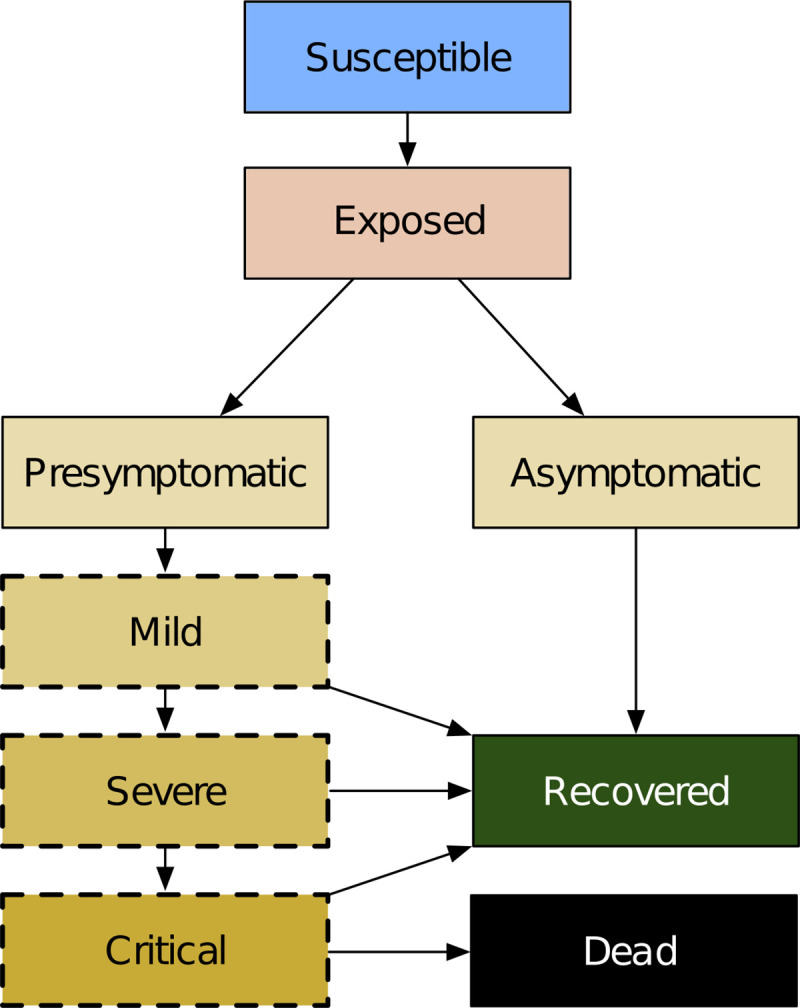
\includegraphics[scale=0.6]{covasim-compartments.jpg}
        \caption[Agent states used in Covasim]{Agent states used in Covasim \cite{kerrCovasimAgentbasedModel2021}}
        \label{fig:covasim-compartments}
    \end{figure}

    \framebreak

    \begin{figure}[!htb]
        \centering
        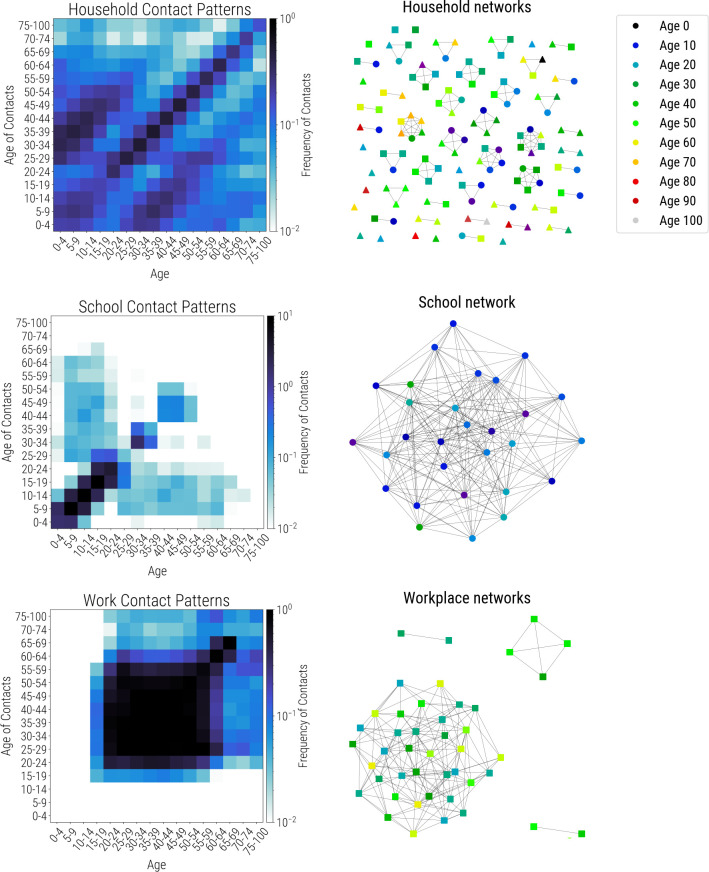
\includegraphics[scale=0.8]{covasim-networks.jpg}
        \caption[Transmission networks used in Covasim]{Transmission networks used in Covasim \cite{kerrCovasimAgentbasedModel2021}}
        \label{fig:covasim-networks}
    \end{figure}

    \framebreak

    \begin{exampleblock}{Pros}
    \begin{itemize}
        \item Explainable
        \item Based on many years of research
        \item Easy to understand and implement
    \end{itemize}
    \end{exampleblock}

    \begin{alertblock}{Cons}
    \begin{itemize}
        \item Low representational capabilities
        \item The represented dynamics are stationary
        \item Unrealistic assumptions about real-world scenarios
    \end{itemize}
    \end{alertblock}

\end{frame}

\begin{frame}[allowframebreaks]{Data-driven models}

    ARIMA models \cite{ceylanEstimationCOVID19Prevalence2020,singhPredictionCOVID19Pandemic2020,ribeiroShorttermForecastingCOVID192020}
    \begin{itemize}
        \item Suitable for modeling changing trends, periodic changes, and random noises
        \item Suitable for different types of data
        \item Can capture temporal dependency of time series
    \end{itemize}

    \framebreak

    Deep-learning models \cite{chimmulaTimeSeriesForecasting2020,shahidPredictionsCOVID19Deep2020,ramchandaniDeepCOVIDNetInterpretableDeep2020}
    \begin{itemize}
        \item \gls{LSTM}
        \item \gls{Bi-LSTM}
        \item \gls{GRU}
    \end{itemize}

    \framebreak

    \begin{exampleblock}{Pros}
    \begin{itemize}
        \item High prediction accuracy
        \item Allow for modeling without needing domain knowledge
    \end{itemize}
    \end{exampleblock}

    \begin{alertblock}{Cons}
    \begin{itemize}
        \item Unexplainable
        \item Relied on large amount of data
        \item Inability to capture the true disease dynamics
    \end{itemize}
    \end{alertblock}

\end{frame}

\begin{frame}[allowframebreaks]{Novel compartmental models}

    Mitigate the disadvantages of compartmental models by incorporating covariates
    \begin{itemize}
        \item using predefined functions based on domain knowledge
        \item using neural networks
    \end{itemize}

    \framebreak

    \begin{figure}[!htb]
        \centering
        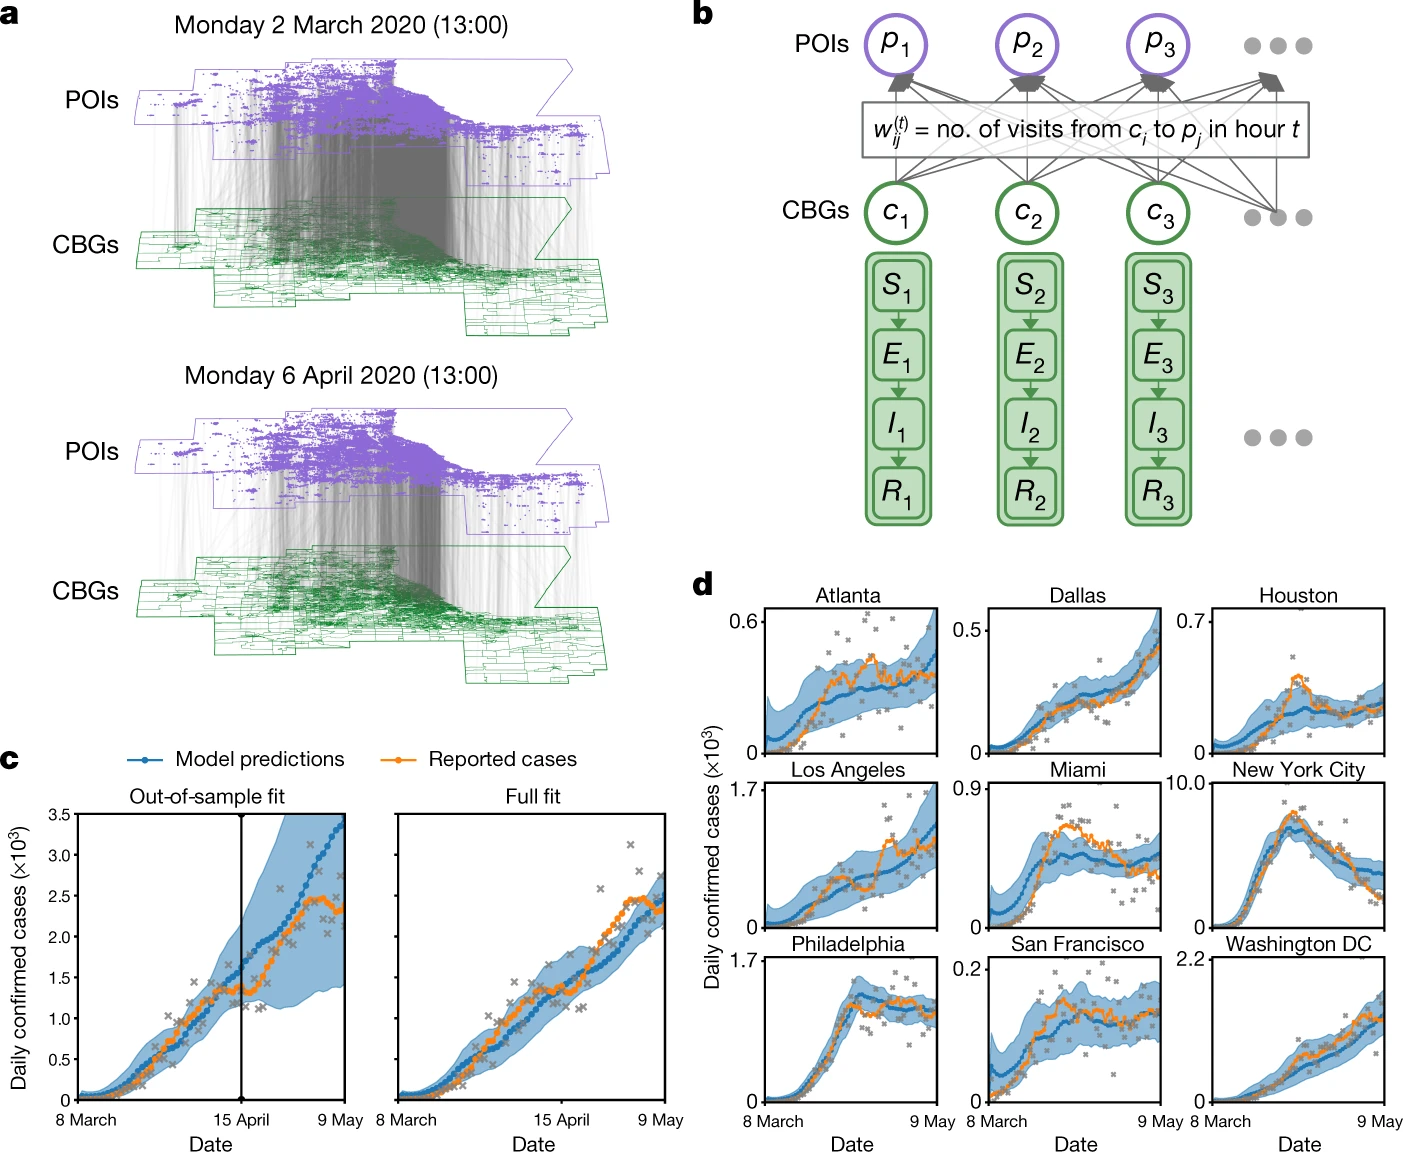
\includegraphics[scale=0.2]{nature-chang-mobility-covid19.png}
        \caption[SEIR model weighted using complex mappings of point-to-point mobility data]{SEIR model weighted using complex mappings of point-to-point mobility data \cite{changMobilityNetworkModels2021}}
        \label{fig:nature-chang-mobility-covid19}
    \end{figure}

    \begin{figure}[!htb]
        \centering
        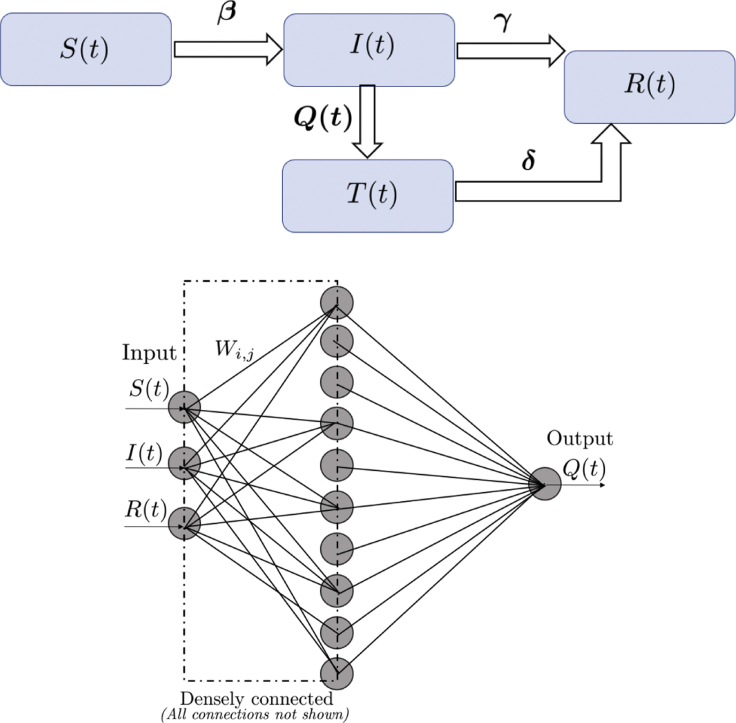
\includegraphics[width=0.4\linewidth]{mit-dandekar-qsir.jpg}
        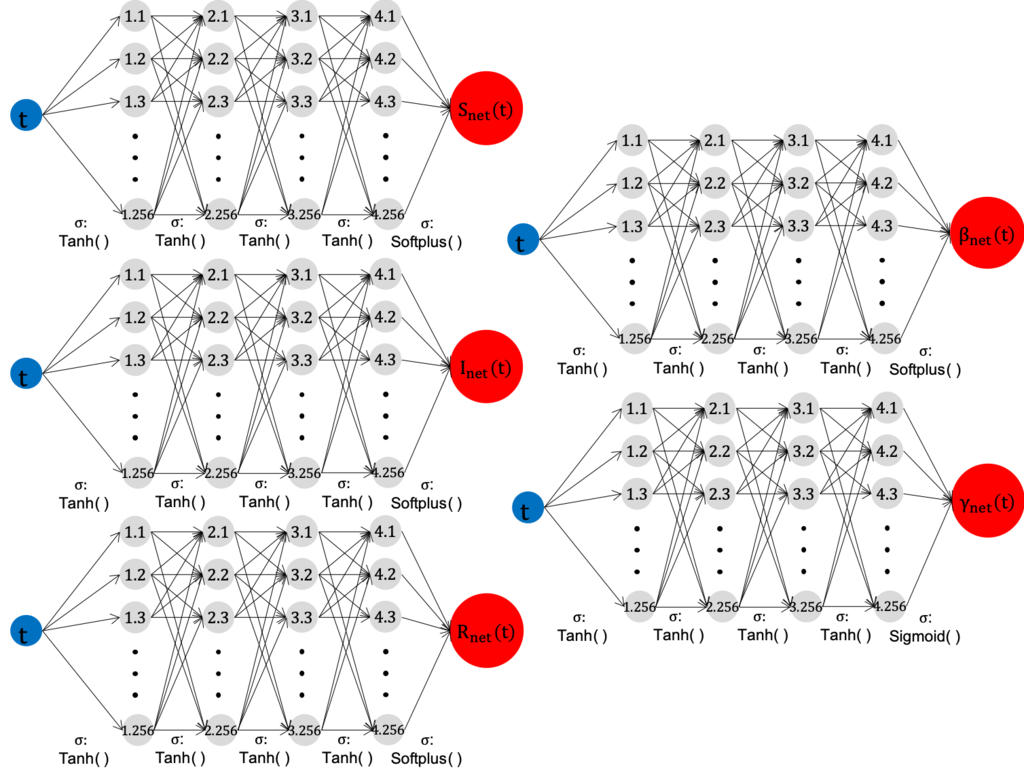
\includegraphics[width=0.4\linewidth]{jung-sir-pinn.png}
        \caption[Using neural networks to predicts the parameters for compartmental models]{Using neural networks to predicts the parameters for compartmental models. On the left is the schematic for the QSIR model \cite{dandekarMachineLearningAidedGlobal2020a}, on the right is the schematic for the time-dependent SIR model \cite{jungRealWorldImplicationsRapidly2020}.}
        \label{fig:compartmentals-models-with-neural-networks}
    \end{figure}

\end{frame}

\subsection{Artificial Neural Network}

\begin{frame}[allowframebreaks]{Multi-layer perceptron}

    \begin{figure}[h]
        \centering
        \begin{neuralnetwork}
            \newcommand{\nodex}[2]{$x_#2$}
            \newcommand{\nodey}[2]{$y_#2$}

            \inputlayer[count=3, bias=false, title={Input\\layer}, text=\nodex]
            \hiddenlayer[count=4, bias=false, title={Hidden\\layer}]
            \linklayers[title=$W_1$]
            \hiddenlayer[count=4, bias=false, title={Hidden\\layer}]
            \linklayers[title=$W_2$]
            \outputlayer[count=2, bias=false, title={Output\\layer}, text=\nodey]
            \linklayers[title=$W_3$]
        \end{neuralnetwork}
        \caption[Illustration of a multi-layer perceptron]{Graph representation of a multi-layer perceptron with four layers}
        \label{fig:multi-layer-perceptron}
    \end{figure}

    \framebreak

    \begin{figure}[h]
        \centering
        \begin{neuralnetwork}
            \newcommand{\nodex}[2]{$x_#2$}
            \newcommand{\nodey}[2]{$y_#2$}

            \inputlayer[count=3, bias=false, title={Input\\layer}, text=\nodex]
            \hiddenlayer[count=4, bias=false, title={Hidden\\layer}]
            \linklayers[title=$\frac{\delta a^1}{\delta W^1}$,style={<-,draw=red}]
            \hiddenlayer[count=4, bias=false, title={Hidden\\layer}]
            \linklayers[title=$\frac{\delta a^2}{\delta W^2}$,style={<-,draw=red}]
            \outputlayer[count=2, bias=false, title={Output\\layer}, text=\nodey]
            \linklayers[title=$\frac{\delta a^3}{\delta W^3}$,style={<-,draw=red}]
        \end{neuralnetwork}
        \caption[Illustration of a multi-layer perceptron]{Graph representation of the back-propagation algorithm on a multi-layer perceptron with four layers}
        \label{fig:multi-layer-perceptron-backpropagation}
    \end{figure}

\end{frame}

% \subsection{Data-driven models}
% \begin{frame}{Data-driven models}
% \begin{itemize}
%     \item Statistical models
%     \item Deep-learning models
% \end{itemize}
% \end{frame}

% \subsection{Data-driven compartmental models}

% \begin{frame}{Data-driven compartmental models}
% \begin{itemize}
%     \item Informed with covariates

%     \item Informed with neural networks
% \end{itemize}
% \end{frame}

% \subsection{Scientific machine learning}
